\chapter{Conclusions}
\label{chap:Conclusions}

%Summary: summarize work and impact, describe directions for further work, describe how this provides a framework for an end to end solution in radio astronomy as well as other domain specific applications
%Goal: show everything worked and was awesome
%State: needs results, should be quick to write but difficult to write now

\section{Summary}
%TODO: explain this in text
\begin{figure}[ht!]
  \centering
    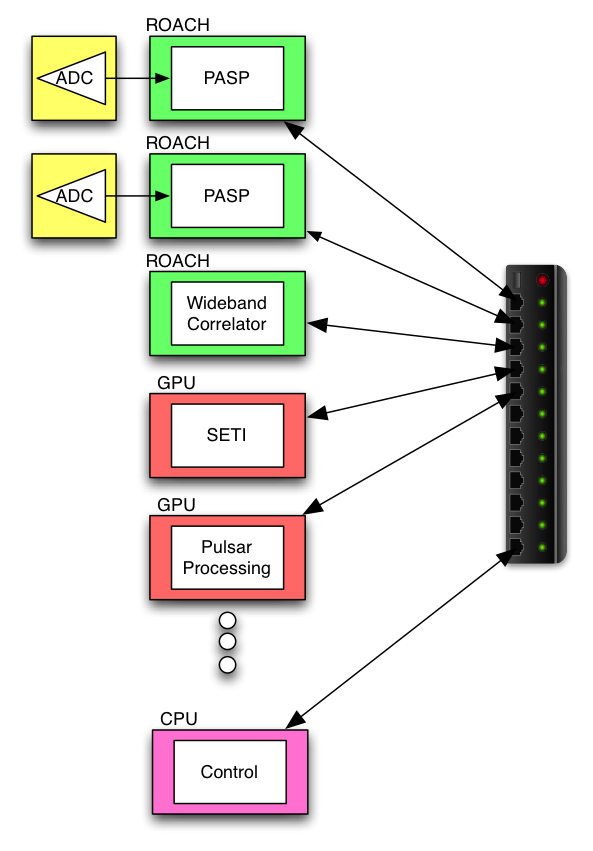
\includegraphics[width=0.5\textwidth]{Images/C5/universal_arch.png}
  \caption{A potential architecture for multiple scientific instruments simultaneously processing data from the same telescope}
  \label{fig: C5/universal_arch.png}
\end{figure}

\section{Future Work}
This success of this work opens up a lot of related projects to improve upon the existing mapping capabilities.
While the instruments developed with ORCAS are designed for radio astronomy, ORCAS was developed as a general purpose tool and the expansion of the instrument set into other fields would provide interesting new challenges.
The existence of a DSP library and benchmarks would make it easy to transition to other DSP applications.

There are also improvements that can be made to the model, but they need to be balanced with the ILP to ensure fast runtimes.
As telescopes get larger, a single computational block may need to span multiple boards.
As we saw in the FX Correlator case study, this is going to be the case for the X-Engine in the near future.
Simply supporting that capability would be useful, but it would be better if model was able to determine how to split these blocks between boards.

%Do a better job of preserving symmetry



%Design interconenct

\section{Conclusions}